\documentclass[11pt,a4paper]{article}
\usepackage[margin=23mm]{geometry}
\usepackage[T1]{fontenc}
\usepackage{lmodern}
\usepackage{hyperref}
\usepackage{tikz}
\usetikzlibrary{positioning,arrows.meta}
\title{Core distributed admission: approved correction}
\date{Created-at: 2026-09-05 19:21 CEST}
\begin{document}
\maketitle
\paragraph{Authorization.}
User chat token, received before this implementation:
\texttt{APPROVED-CORE-EDIT: distributed-admission-monotone-resume}.
The approving chat turn identifier is not exposed. Scope is the reviewed patch
in reports/distributed-semantics/proposed-admission-fix.patch and its regression
plan. Base: 1befefbaab0b90e1918be533ce35db57cf540d61, own worktree
D:/hnnwork/distributed/core. No push, merge or release.
\paragraph{ETA.}
20--35 minutes: apply the reviewed correction, wire the existing seven cases,
check checkpoint retention, run focused and full Core verification on Amaterasu,
update status and retain exact evidence. The earlier clean CPU build took about
83 seconds; new compilation and Clippy are allowed several minutes each.
\paragraph{Ownership and discovery.}
Core owns TransactionAssembler, SnapshotVersion and the public wire facade.
Reuse their existing implementation and test harness. The baseline already
reproduced four failures through valid wire messages. No worker-side IR, new
codec, transport, dependency or numerical implementation is introduced.
\paragraph{Files and protected scope.}
Protected: hymeko\_core/src/ir\_stream/assembler.rs only: monotone target guard,
private established-version flag, equal-version unknown-identity recovery and
corresponding contract comments. Public signatures and wire format unchanged.
Move reports/distributed-semantics/admission\_probe.rs to
hymeko\_core/tests/ir\_stream\_admission.rs; register it in
hymeko\_core/tests/mod.rs. Add focused reset/known-identity cases using that same
producer helper. Add this plan quartet, reports/2026-09-05-distributed-admission-fix.md
and reports/distributed-admission-fix/ evidence. Update .gitattributes,
docs/unified-ir-architecture.md, docs/hypergraph-synchronization.md and
docs/verification/unified-ir/requirements.md to cite observed correction status.
The preceding audit report, Lean source, baseline logs and manifest remain
historical evidence at 1befefb; the probe move is explicit in the new manifest.
\paragraph{Verification.}
First the seven original cases on the corrected Core, then reset/identity
retention and the existing assembler suite. Run Core release tests, workspace
formatting and all-target Clippy in the existing bounded Docker SDK on Amaterasu.
Build a clean-revision image and retain its source hashes and command exits.
Recheck the unchanged 19 Lean theorems separately. No claim of whole-Rust formal
refinement, durable IR installation, network liveness, GPU retirement or speedup.
\paragraph{Performance and production risks.}
The added admission checks are constant-size comparisons; bounded staging and
replay behavior must remain in force, including unknown-identity traffic and
reset. Existing resource-limit tests remain the acceptance guard for hostile
inputs. At most 16 GiB memory, equal memory+swap quota, six CPUs; no VAS cap.
Use the existing stage RSS/wall-time runner. Small probes are not benchmarks.
\paragraph{Acceptance and rollback.}
Four baseline failures must become PASS without weakening their expectations;
all planned checks must be reported, including any failure. The original user
worktree is untouched. Local thematic implementation and evidence commits are
authorized; include the token in the implementation commit footer. Revert only
the scoped implementation commit to roll back; preserve original counterexamples.
Dependency/CI, browser and consumer experiments remain later integration stages.
\begin{center}
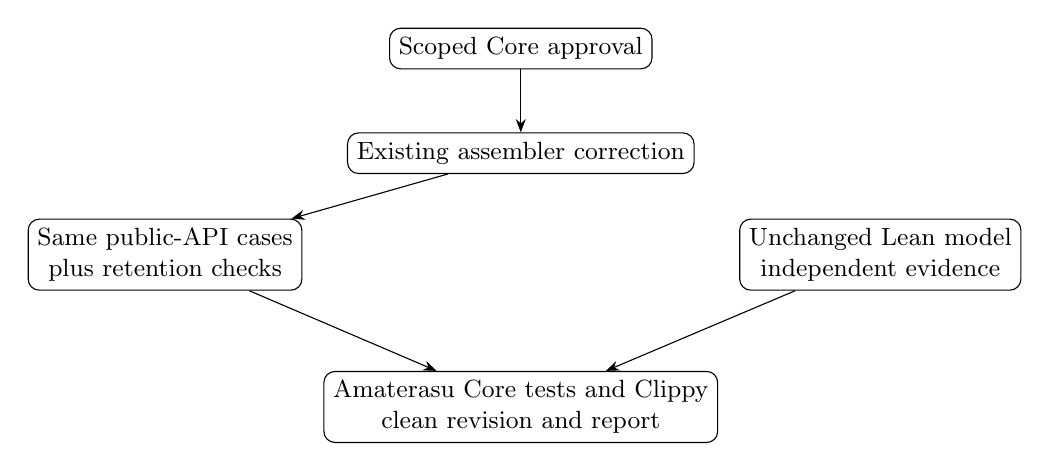
\begin{tikzpicture}[node distance=8mm, every node/.style={draw,rounded corners,align=center,font=\small}, >=Stealth]
\node (approval) {Scoped Core approval};
\node (fix) [below=of approval] {Existing assembler correction};
\node (tests) [below left=of fix] {Same public-API cases\\plus retention checks};
\node (proof) [below right=of fix] {Unchanged Lean model\\independent evidence};
\node (result) [below=25mm of fix] {Amaterasu Core tests and Clippy\\clean revision and report};
\draw[->] (approval) -- (fix);
\draw[->] (fix) -- (tests);
\draw[->] (tests) -- (result);
\draw[->] (proof) -- (result);
\end{tikzpicture}
\end{center}

\end{document}
